% Template for documenting your Arduino projects
% Author:   Luis José Salazar-Serrano
%           totesalaz@gmail.com / luis-jose.salazar@icfo.es
%           http://opensourcelab.salazarserrano.com
%%% Template based in the template created by Karol Kozioł (mail@karol-koziol.net)

\def \TITLE     {Blinking LED}
\def \AUTHOR    {Suka Isnaini, COHERENCE, Kenzanin@gmail.com}
\def \SUBJECT   {ESP8266}
\def \KEYWORDS  {Python, Python-PIP, PlatformIO}

\documentclass[a4paper,11pt]{article}

\usepackage[T1]{fontenc}
\usepackage[utf8]{inputenc}
\usepackage{graphicx}
\usepackage{xcolor}

\renewcommand\familydefault{\sfdefault}
\usepackage{tgheros}
\usepackage[defaultmono]{droidmono}

\usepackage{amsmath,amssymb,amsthm,textcomp}
\usepackage{enumerate}
\usepackage{multicol}
\usepackage{tikz}
\usepackage{courier}

\usepackage{geometry}
\geometry{total={210mm,297mm},
left=25mm,right=25mm,%
bindingoffset=0mm, top=20mm,bottom=20mm}

%\linespread{1.3}
\newcommand{\linia}{\rule{\linewidth}{0.5pt}}

% my own titles
\makeatletter
\renewcommand{\maketitle}{
\begin{center}
\vspace{2ex}
{\huge \textsc{\@title}}
\vspace{1ex}
\\
\linia\\
\@author \hfill \@date
\vspace{4ex}
\end{center}
}
\makeatother
%%%

% custom footers and headers
\usepackage{fancyhdr}
\pagestyle{fancy}
\lhead{}
\chead{}
\rhead{}
\lfoot{\TITLE}
\cfoot{}
\rfoot{Page \thepage}
\renewcommand{\headrulewidth}{0pt}
\renewcommand{\footrulewidth}{0pt}
%

% code listing settings

\usepackage{listings}

\lstset{%
  basicstyle=\footnotesize\ttfamily,       
  breakatwhitespace=false,         
  breaklines=true,                 
  captionpos=b,                   
  frame=single,                    
  keepspaces=true,                 
  tabsize=2,                       
  title=\lstname,
  emphstyle=\bfseries\color{blue}%  style for emph={} 
} 


%% language specific settings:
\definecolor{dkgreen}{rgb}{0,0.6,0}
\definecolor{dred}{rgb}{0.545,0,0}
\definecolor{dblue}{rgb}{0,0,0.545}
\definecolor{lgrey}{rgb}{0.9,0.9,0.9}
\definecolor{gray}{rgb}{0.4,0.4,0.4}
\definecolor{darkblue}{rgb}{0.0,0.0,0.6}
\lstdefinestyle{C++}{%
    language = C++,
    morecomment=[l]{//},%             treat // as comments
    morecomment=[s]{/*}{*/},%         define /* ... */ comments
    emph={HIGH, OUTPUT, LOW},%        keywords to emphasize
    backgroundcolor=\color{lgrey},  
    basicstyle=\footnotesize \ttfamily \color{black} \bfseries,   
    commentstyle=\color{dkgreen},   
    deletekeywords={...},          
    escapeinside={\%*}{*)},                  
    keywordstyle=\color{red},  
    morekeywords={}, 
    identifierstyle=\color{black},
    stringstyle=\color{blue},      
    numbers=left,                 
    numbersep=5pt,                  
    numberstyle=\tiny\color{black}, 
    rulecolor=\color{black},        
    showspaces=false,               
    showstringspaces=false,        
    showtabs=false,                
    stepnumber=1,                   
}

\lstdefinestyle{bash}{%
    language=bash,
    backgroundcolor=\color{lgrey},  
    basicstyle=\footnotesize \ttfamily \color{black} \bfseries,   
    commentstyle=\color{dkgreen},   
    deletekeywords={...},          
    keywordstyle=\color{red},  
    morekeywords={mkdir, pio}, 
    identifierstyle=\color{black},
    stringstyle=\color{blue},      
    numbers=left,                 
    numbersep=5pt,                  
    numberstyle=\tiny\color{purple}, 
    rulecolor=\color{black},        
    showspaces=false,               
    showstringspaces=false,        
    showtabs=false,                
    stepnumber=1,                       
}

% tambahan
\usepackage{inconsolata}
\usepackage{svg}
\usepackage{hyperref}
\hypersetup{colorlinks=true,allcolors=blue}
\usepackage{hypcap}
\hypersetup{
    pdftitle={\TITLE},
    pdfauthor={\AUTHOR},
    pdfsubject={\SUBJECT},
    pdfkeywords={\KEYWORDS},
    bookmarksnumbered=true,     
    bookmarksopen=true,         
    bookmarksopenlevel=1,       
    colorlinks=true,            
    pdfstartview=Fit,           
    pdfpagemode=UseOutlines,    % this is the option you were lookin for
}
\usepackage{datetime}
%%%----------%%%----------%%%----------%%%----------%%%


\begin{document}

\title{\TITLE}

\author{\AUTHOR}

\date{\today}

\maketitle
\tableofcontents
\newpage

\section{Tujuan Percobaan}
Mengatur nyala mati nya LED yang terhubung ke ESP8266, melalui software.

\section{Hasil yang diharapkan}
Led menyala selama 1 detik, mati selama 1 detik dan berulang.

\section{Komponen yang digunakan}
\begin{itemize}
\item 1 pcs Power supply 5v atau bisa dari USB yang terhubung dengan PC.
\item 1 pcs LED merah diffused (yang bright bikin sakit mata).
\item 1 pcs Resistor dengan nilai 1K Ohm.
\end{itemize}

\section{Circuit}
Power Supply 5v hanya dibutuhkan jika rangkaian tidak terbubung dengan USB komputer, jika USB terhubung dengan komputer maka sumber tegangan 5V didapatkan langsung dari port USB komputer. Pada percobaan ini LED terhubung dengan ESP8266 melalui R 1K yang bertujuan untuk membatasi arus yang mengalir pada LED. Lebih lengkap nya bisa dilihat pada Figure~\ref{circuit01}.

\section{Warning}
Jangan sampai terbalik menghubungkan polaritas dari power supply ke ESP8266, kesalahan penyambungan berakibat rusak nya rangkaian ESP8266.

\newpage

\begin{figure}[h]
\centering
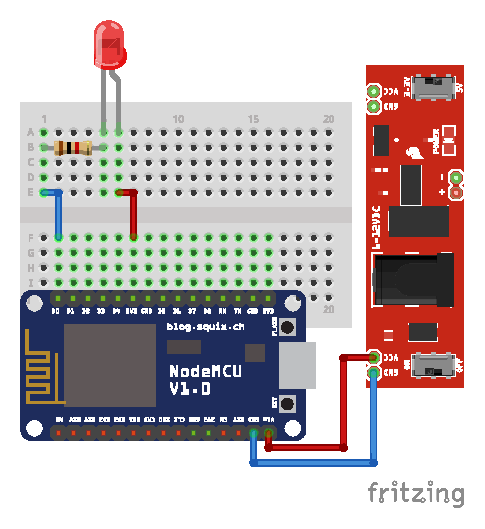
\includegraphics[width=0.9\linewidth]{sch/led_blink_bb}
\caption{Rangkaian LED Blink.}
\label{circuit01}
\end{figure}

\section{Code Description}
Pada Esp8266 terdapat 16 GPIO yang bisa digunakan baik sebagai input atau sebagai output. Percobaan ini menggunakan GPIO D0 yang disetting sebagai output. Sesuai dengan Figure~\ref{circuit01}\ldots{} maka untuk menyalakan LED, D0 harus berada pada kondisi LOW atau 0, sedang untuk menyalakan LED D0 harus pada kondisi HIGH atau 1. Sedangkan untuk durasi nyala dan mati nya LED menggunakan fungsi wait yang telah disediakan oleh OS (Operating System).

\section{Software Code}
Pembuatan software diawali dengan setup project dengan cara menjalankan perintah seperti pada Listing~\ref{setup_project_blink}\ldots{} pada terminal.
\newpage
\begin{lstlisting}[label=setup_project_blink,caption=Setup project blink,style=bash]
$ mkdir led_blink
$ cd led_blink
$ pio init --ide=codeblocks --board=d1 --project-option "framework=esp8266-rtos-sdk"
\end{lstlisting}

Jika tidak ada error maka akan terdapat file platfromio.cbp yang merupakan project file untuk codeblocks. Buka platfromio.cbp dengan codeblocks dan buat file baru dengan nama blink.c yang berisi dengan code seperti pada Listing~\ref{blink-main-c}.

\lstinputlisting[label=blink-main-c,style=C++,caption=Pogram utama LED blink]{src/src/blink.c}

Pastikan semua perintah ditulis dengan benar dan build project, jika tidak ada error yang dilaporkan oleh codeblocks maka project bisa diupload ke board dengan menggunakan perintah

\begin{lstlisting}[label=blink-upload,caption=Upload Project ke board,style=bash]
$ pio --target upload
\end{lstlisting}

\section{Analisa}
Pogram Listing~\ref{blink-main-c}\ldots{} pada dasarnya hanya membuat D0 menjadi output, dan memberikan fungsi tunda nyala dan mati pada LED. Perintah untuk membuat D0 menjadi output terdapat pada baris 53 sampai 58, dan untuk fungsi tunda 1 detik terdapat pada baris 64 dan 66.

\section{Pengembangan dan latihan}
\begin{itemize}
\item Ganti rangkaian dan pogram untuk D1
\item Ganti delay dari 1s ke 500ms
\end{itemize}

\end{document}
